\documentclass{article}
\usepackage[utf8]{inputenc}
\usepackage{hyperref}
\usepackage{graphicx}
\usepackage{authblk}
\usepackage[margin=1in]{geometry}
\usepackage{subfig}

\newcommand{\rcs}{\chi^2_\nu}
\newcommand{\cs}{\chi^2}

\title{Developing CCD Camera Linearity Corrections for the Fredonia Observatory}
\author[1]{\sc{Zach Yek}}
\author[1]{\sc{Michael M. Dunham}}
\affil[1]{Department of Physics, State University of New York at Fredonia, 280 Central Ave, Fredonia, NY 14063, USA}
\date{July 2020}

\begin{document}

\maketitle

\begin{abstract}
    The relationship between a CCD camera's pixel counts vs exposure time tends to divert from linearity as it approaches the saturation limit. To correct for this, we established a linearity correction calibration procedure for the CCD camera in the Fredonia observatory. Based on testing multiple different functions, we have determined the best linearity correction to add would be a constant offset with a break point at 28000~counts.
\end{abstract}

\section{Introduction}
For any given camera that is exposed to a constant illumination, we expect the relationship between the pixel's counts (the signal received) and the exposure time to be linear up until the saturation limit, but in reality, certain underlying physical characteristics of the camera's sensor tend to cause this relationship to divert from linearity as it approaches its saturation limit\footnote{Further reading available at \href{ https://people.csail.mit.edu/hasinoff/pubs/hasinoff-saturation-2012-preprint.pdf}{https://people.csail.mit.edu/hasinoff/pubs/hasinoff-saturation-2012-preprint.pdf}}. We know that the saturation limit for our telescope's camera is precisely 65535 counts. The goal of this project is to create a linearity correction calibration procedure that can be applied to all science images taken using the camera.

\section{Methods}
We used a constant light source that was directed at the dome wall as the dome was closed, and pointed the telescope at the wall. A sequence of images with increasing exposure times was then taken. Multiple images at each exposure time were taken to reduce uncertainties due to random fluctuations. We also took a sequence of images where the exposure time $t=0$~s to account for the camera's bias\footnote{A bias frame is a zero-length exposure to show any underlying structure in the image from the CCD or electronics.}. The light source was set such that the counts recorded were only a few percent of the saturation level in the shortest integration times measured (which was 0.5~s).

\begin{figure}[!htb]
    \centering
    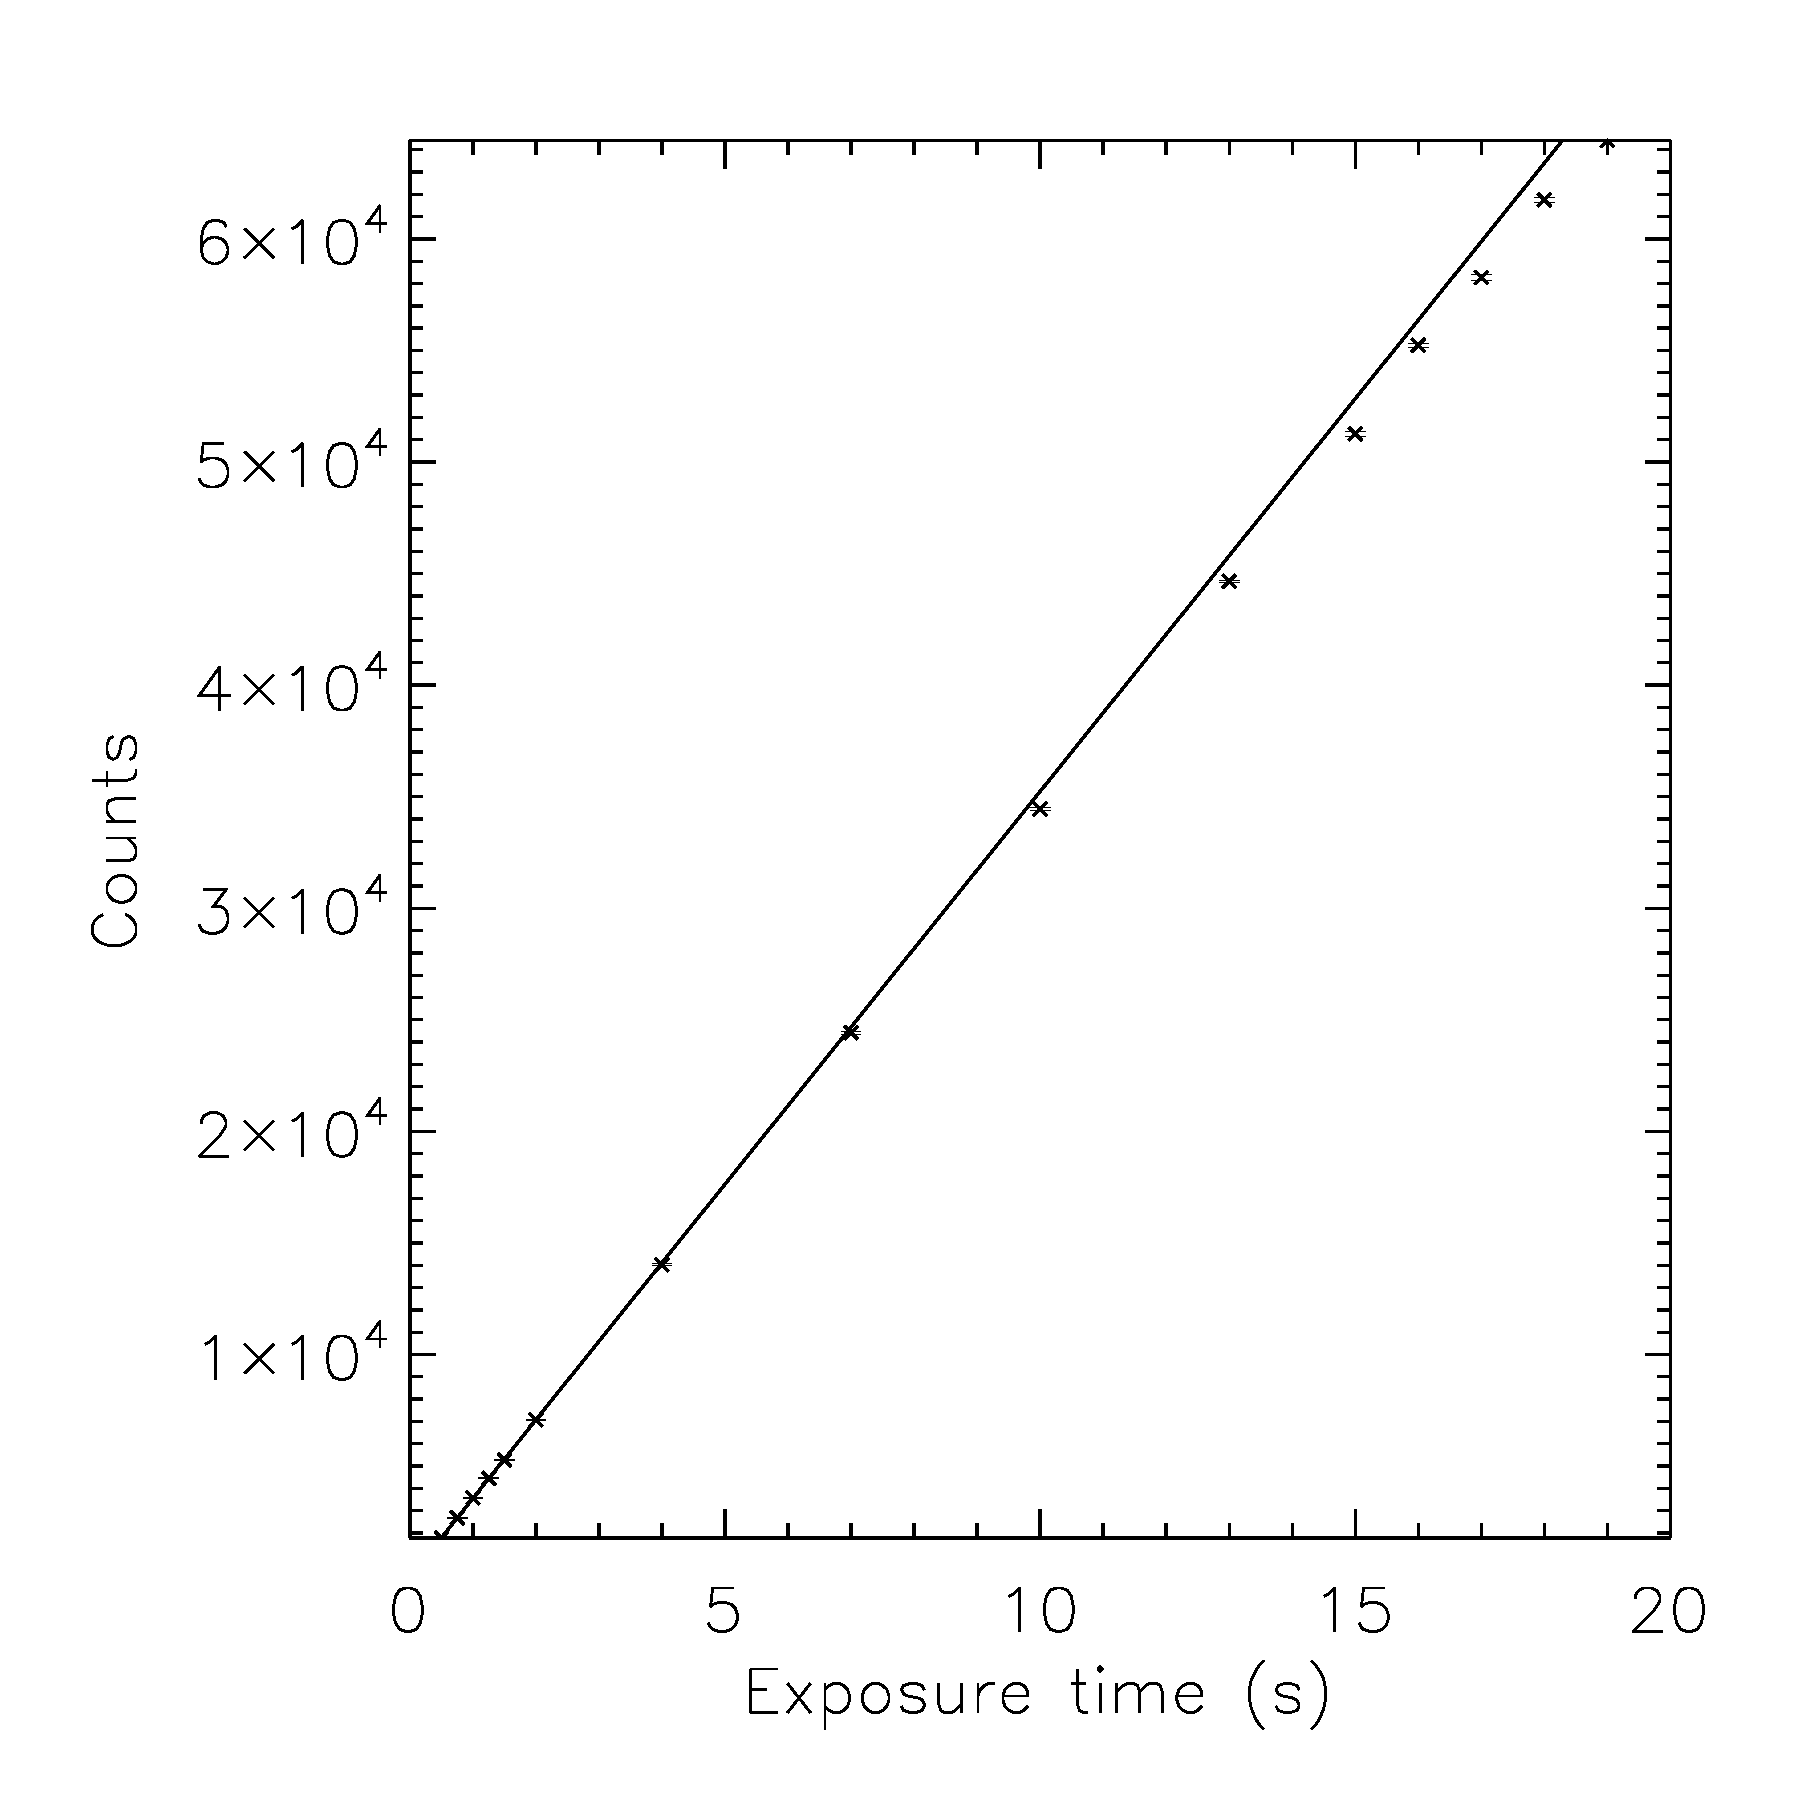
\includegraphics[width=10cm]{exptime_counts_plot.eps}
    \caption{For a randomly selected pixel in the camera array, the counts in each master image is plotted versus the corresponding exposure time for that master image. Note that the linear relationship line is fitted to the shortest 5 exposure times, as we're confident that the camera is linear at such low counts.}
    \label{fig1}
\end{figure}

Then, we averaged all the images at a given exposure time together to create a master image for each exposure time. For each pixel in the camera array, we plotted the counts in each master image versus its exposure time, and then fit a linear relationship to the shortest 5 exposure times, as we're confident that the camera is linear at such low counts. Figure \ref{fig1} is an example of one such plot.

\begin{figure}[!htb]
    \centering
    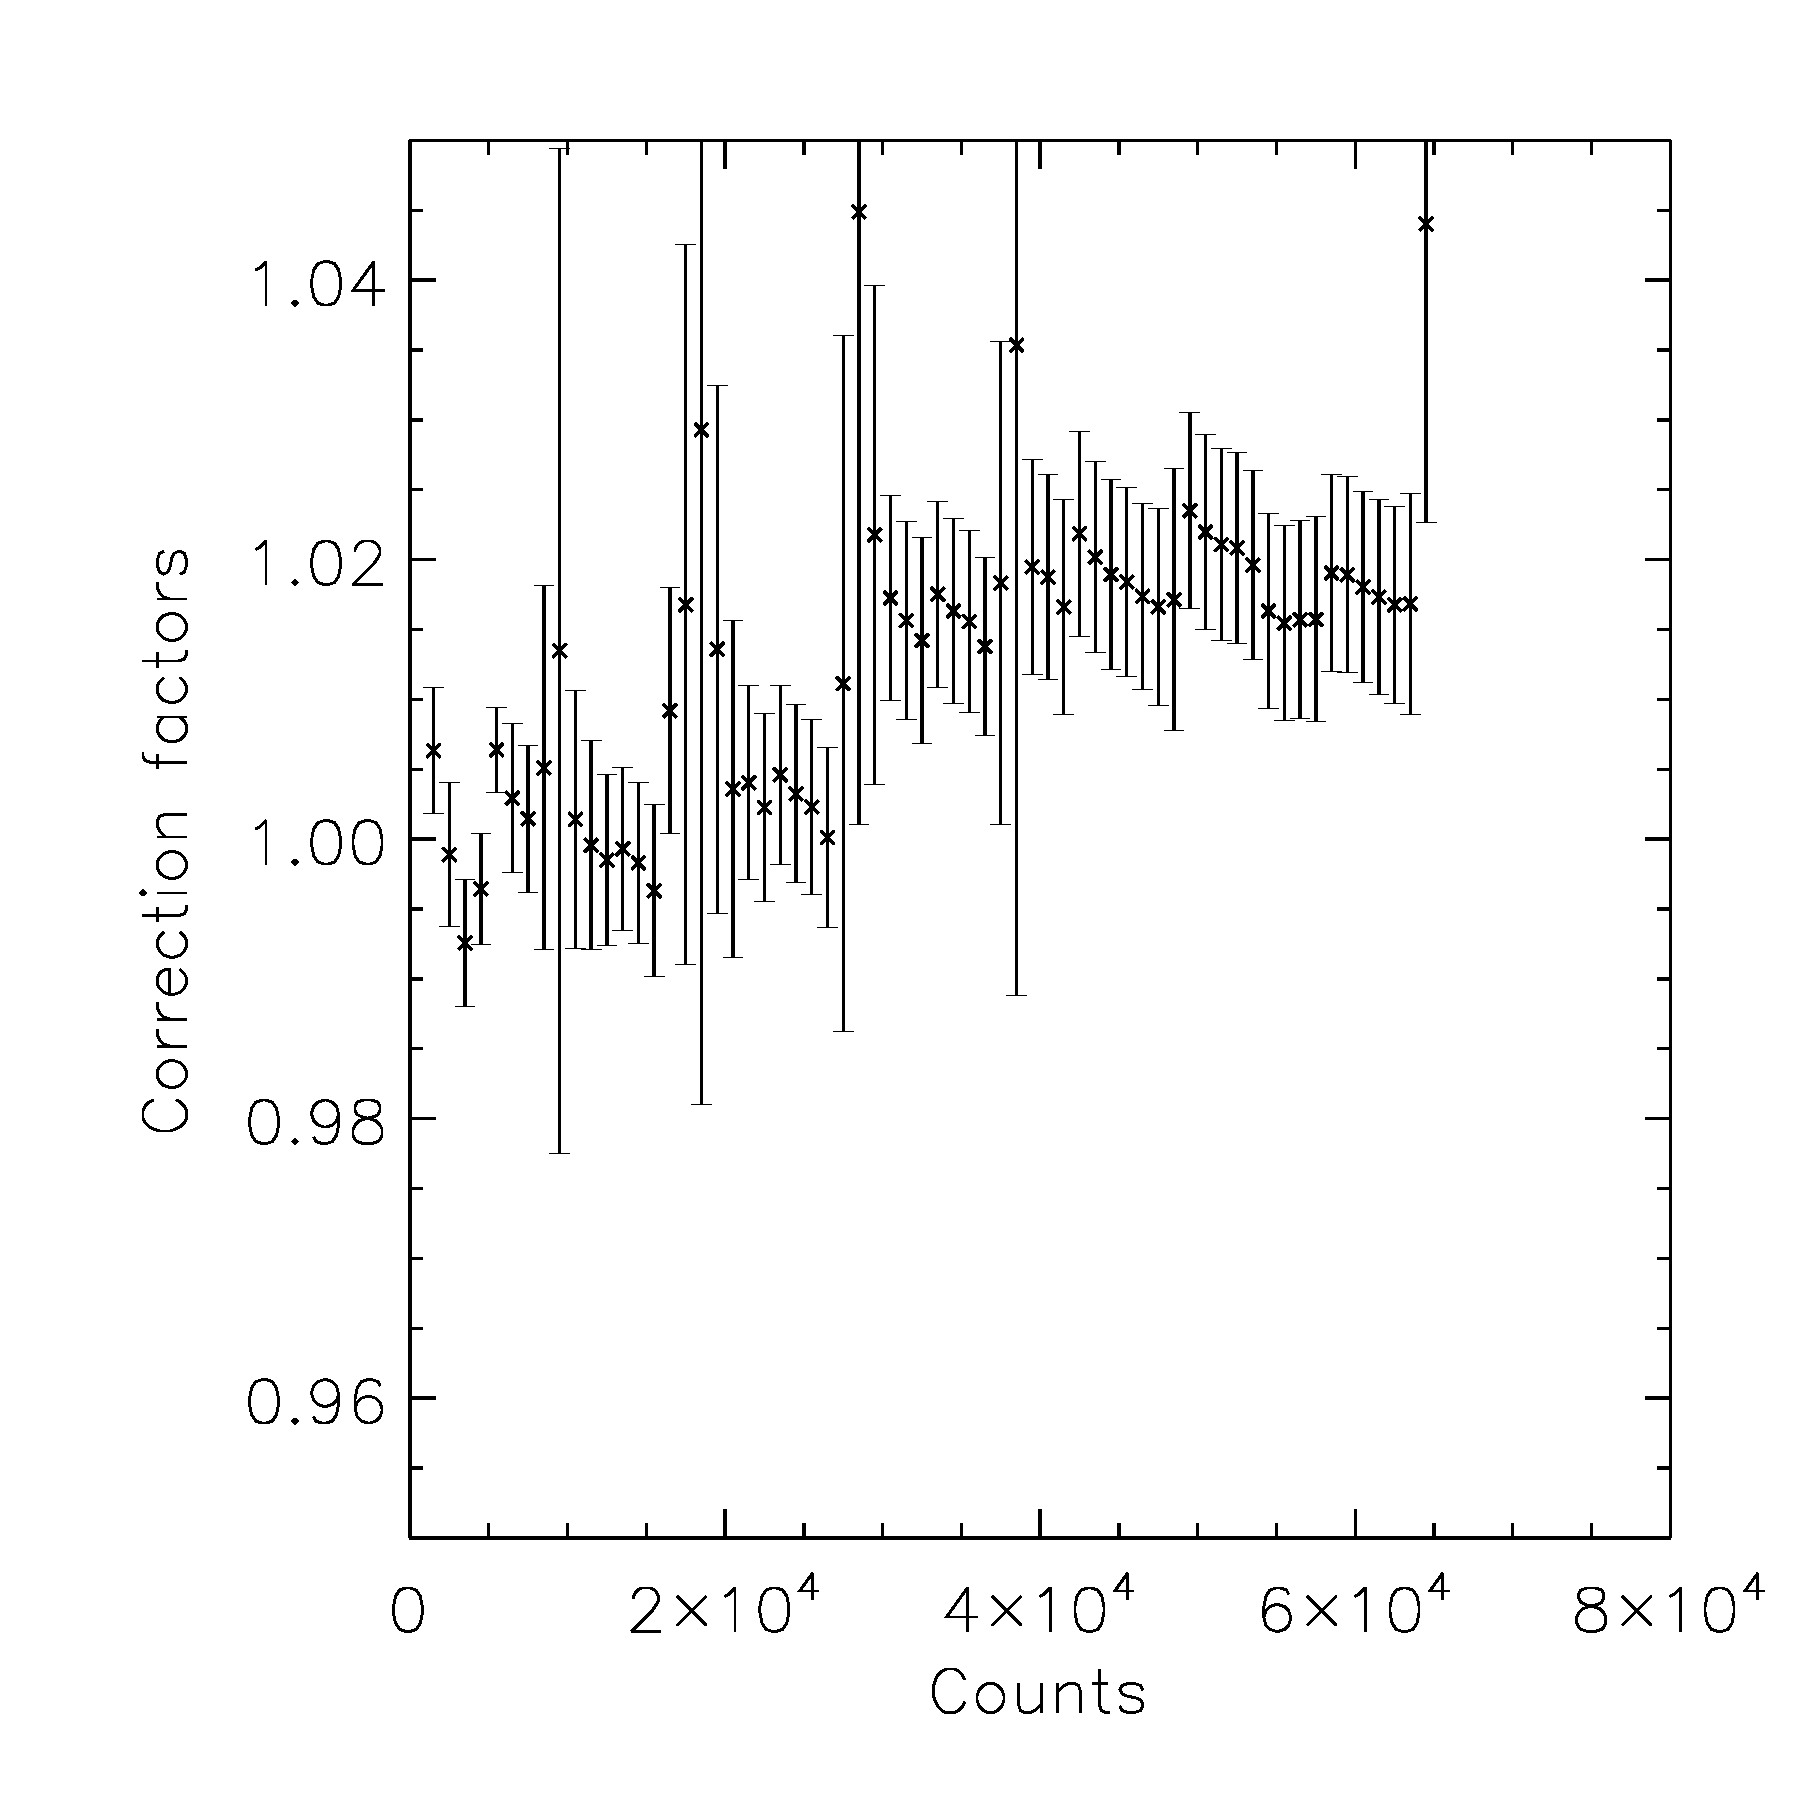
\includegraphics[width=10cm]{counts_crf_plot.eps}
    \caption{Binned correction factors vs measured counts, where the correction factors for each data point are calculated by dividing the expected counts from the linear fit in Figure \ref{fig1}, by the measured counts from the averaged images; the results from all the pixels were combined together, and binned into measured counts bins with a bin size of 1000 counts, with the error bars showing the standard deviation of the data points in each bin. We note here that the correction factors for our telescope's camera range from 2-4\% even at higher exposure times, indicating that the camera is remarkably linear even while it's approaching saturation.}
    \label{fig2}
\end{figure}

From there, we calculated linearity correction factors for each data point by dividing the expected counts from the linear fit by the measured counts from the averaged images. We combined the results from all the pixels together, sorting all of the calculated correction factors into bins based on the measured counts each correction factor applies to. Figure \ref{fig2} displays the binned results, using a bin size of 1000 counts. The plotted data points show the mean correction factor in each bin, and the error bars show the standard deviation in each bin.

After that, we visually identified three possible functions that might be a good fit to Figure \ref{fig2}:
\begin{enumerate}
    \item a straight line function $f(x)=mx+c$, where $c$ is some constant;
    \item a square root function $f(x)=A\sqrt{x}+d$, where $A,d$ are constants;
    \item a piecewise function $f(x)=a$ when $0<x<p$, $f(x)=b$ when $p\leq x<65535$, where $a,b$ are constants, and $p$ is the break point.
\end{enumerate}

Subsequently,
\begin{itemize}
    \item for the straight line function $f(x)=mx+c$, we simply fitted a best-fit line to the weighted data points in Figure \ref{fig2}, where we weighed each data point based on their corresponding standard deviations. 
    \item we linearized $f(x)=A\sqrt{x}+d$ by subtracting $d$ from both sides before squaring the equation to obtain a linear function of $x$. We then fit a best-fit line function to the weighted data points following the same procedures described above.
    \item For the piecewise function, we looped through all possible break points between 0 and 65000~counts, in increments of 1000~counts. For each possible break point, we calculated the weighted mean of the binned correction factors above and below the break point, where the weights were set by the standard deviation in each bin.
\end{itemize}

To test the goodness of each fit, we calculated the reduced-chi squared statistic of all three fits as:

\begin{equation}
    \rcs=\frac{\cs}{\nu},
    \label{eq1}
\end{equation}

\noindent where $\rcs$ is defined as chi-squared $\cs$ per degree of freedom $\nu$. Note that $\cs$ is a weighted sum of squared deviations over all data points $n$:

\begin{equation}
    \cs=\sum_i^n(\frac{O_i-C_i}{\sigma_i})^2,
    \label{eq2}
\end{equation}

\noindent where $O_i$ is the observed data point, $C_i$ is the calculated data point, and $\sigma_i$ is the uncertainty of each data point.

We note that for the piecewise function, we calculated each reduced-chi squared value at every break point using Equations \ref{eq1} and \ref{eq2}, and plotted the reduced-chi squared values vs the break points (see Figure 3c) to identify the break point corresponding to the lowest reduced-chi squared value, which we then used as our best-fit piecewise function.

\section{Results \& Discussions}
The results from Figure \ref{fig2} show that the correction factors for our telescope's camera range from 2-4\% even at higher exposure times, indicating that the camera is remarkably linear even as it approaches saturation. It's useful to note that even if we'd stopped here and provided no corrections for future images, the error would only be on the order of a few percent.
\clearpage
\begin{figure}[!htb]
    \centering
    \subfloat[]{{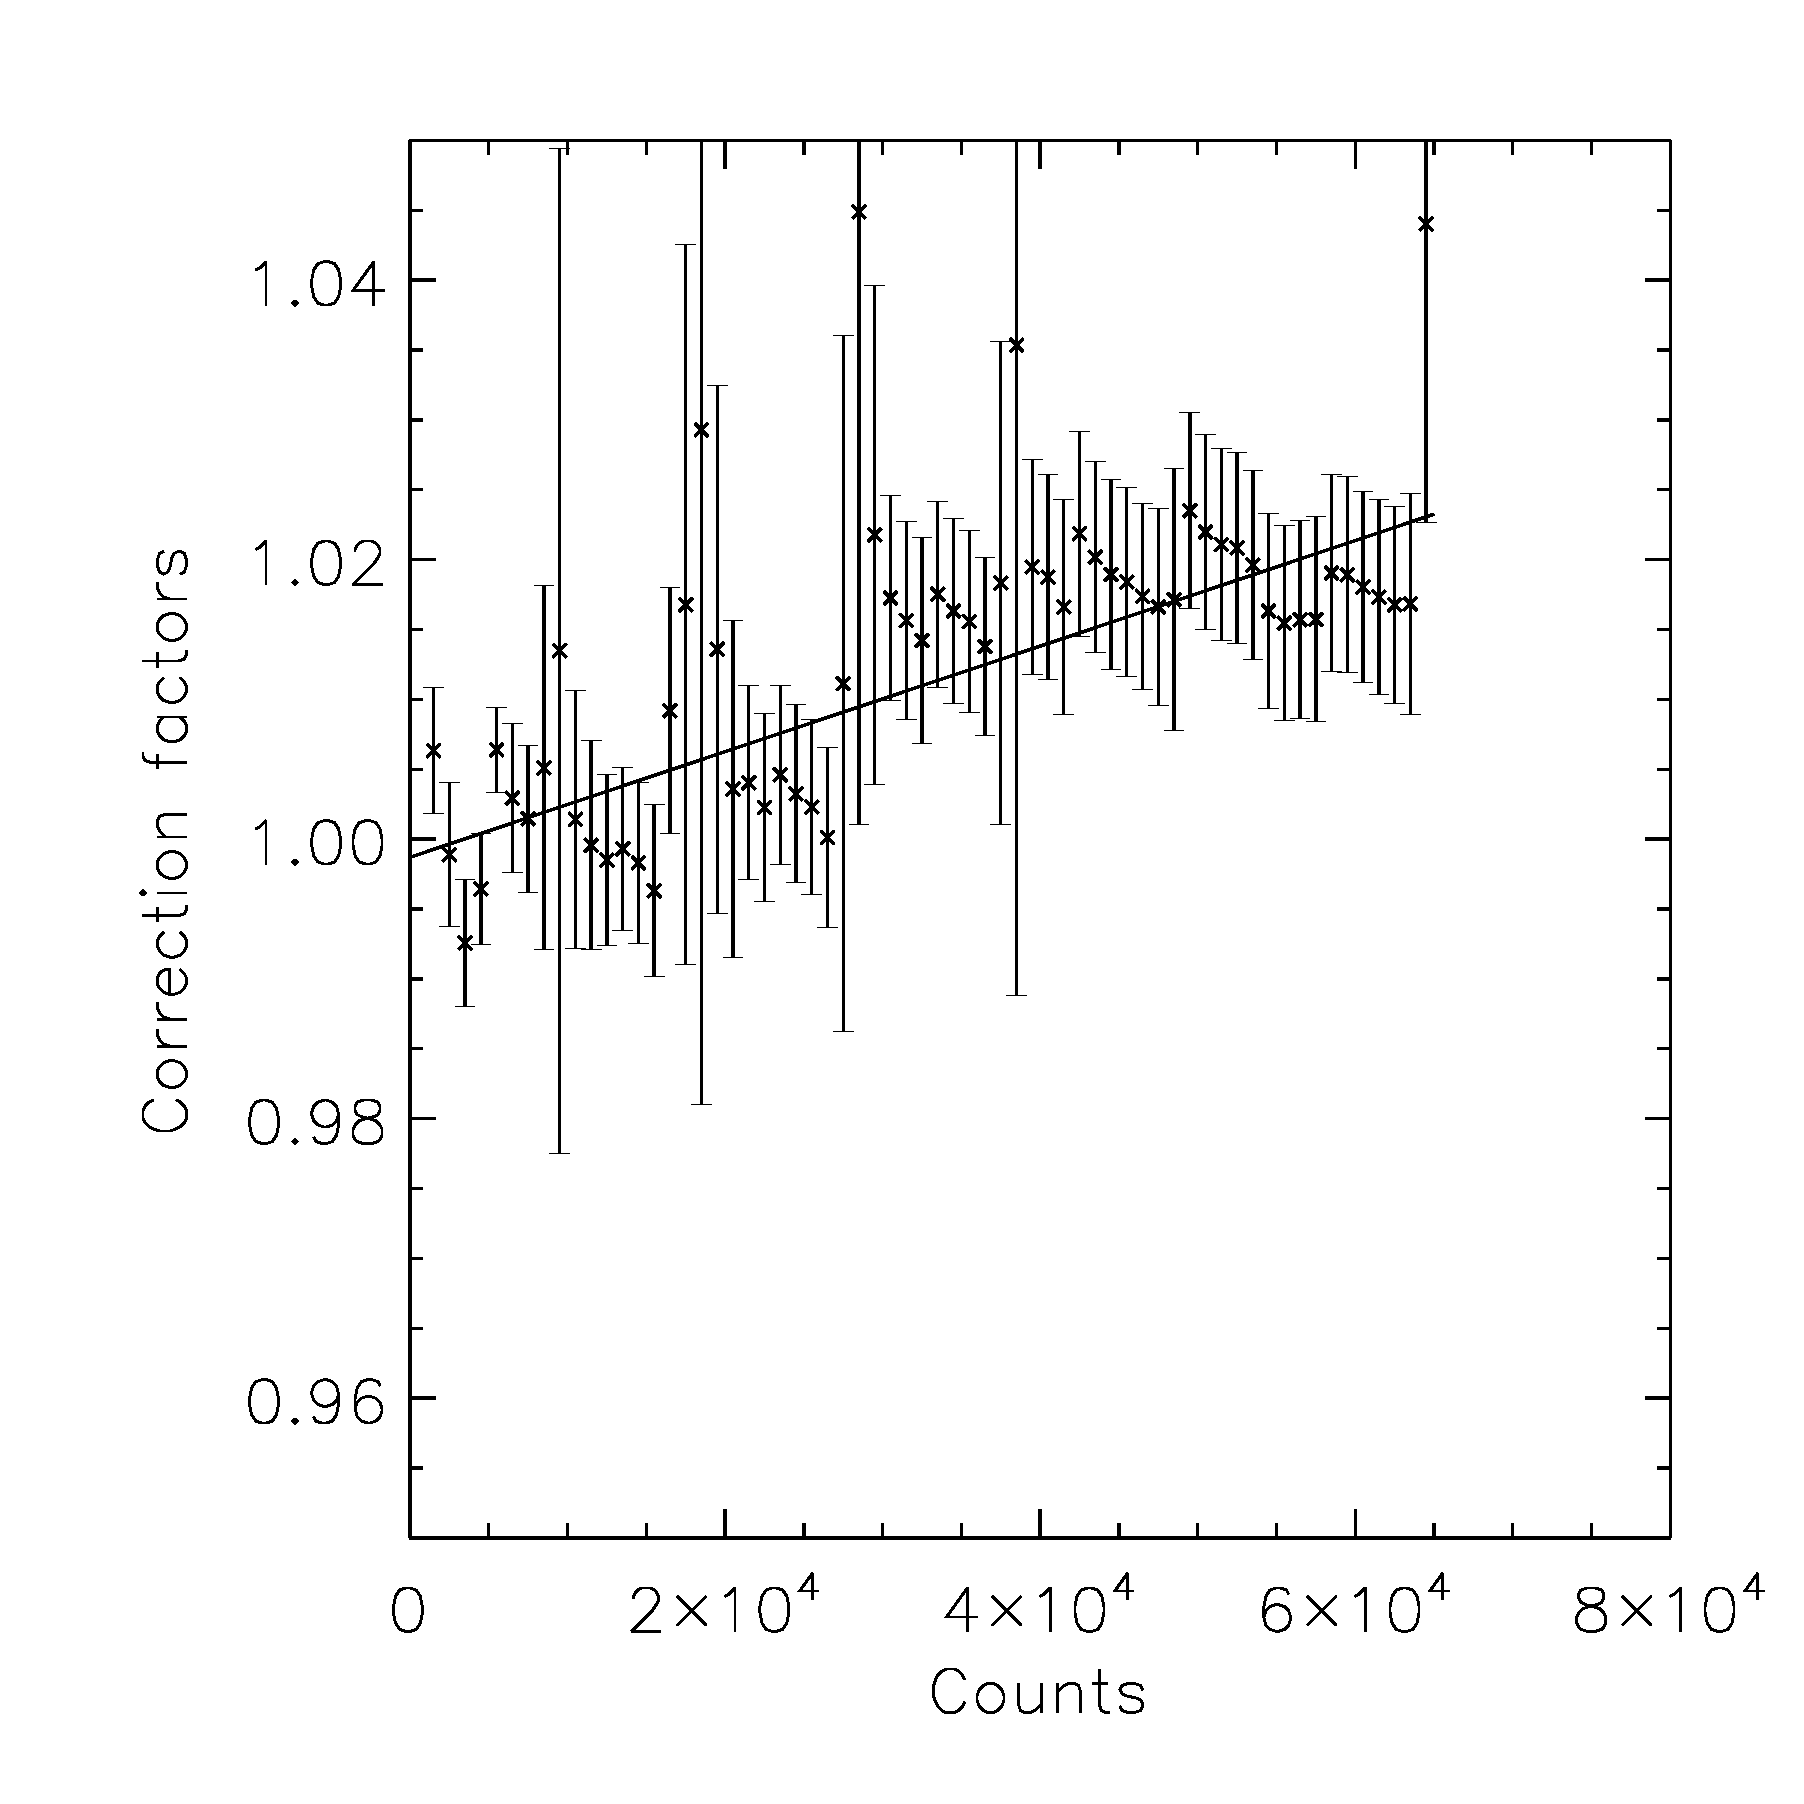
\includegraphics[scale=.25]{mx_c.eps} }}
    \hfill
    \subfloat[]{{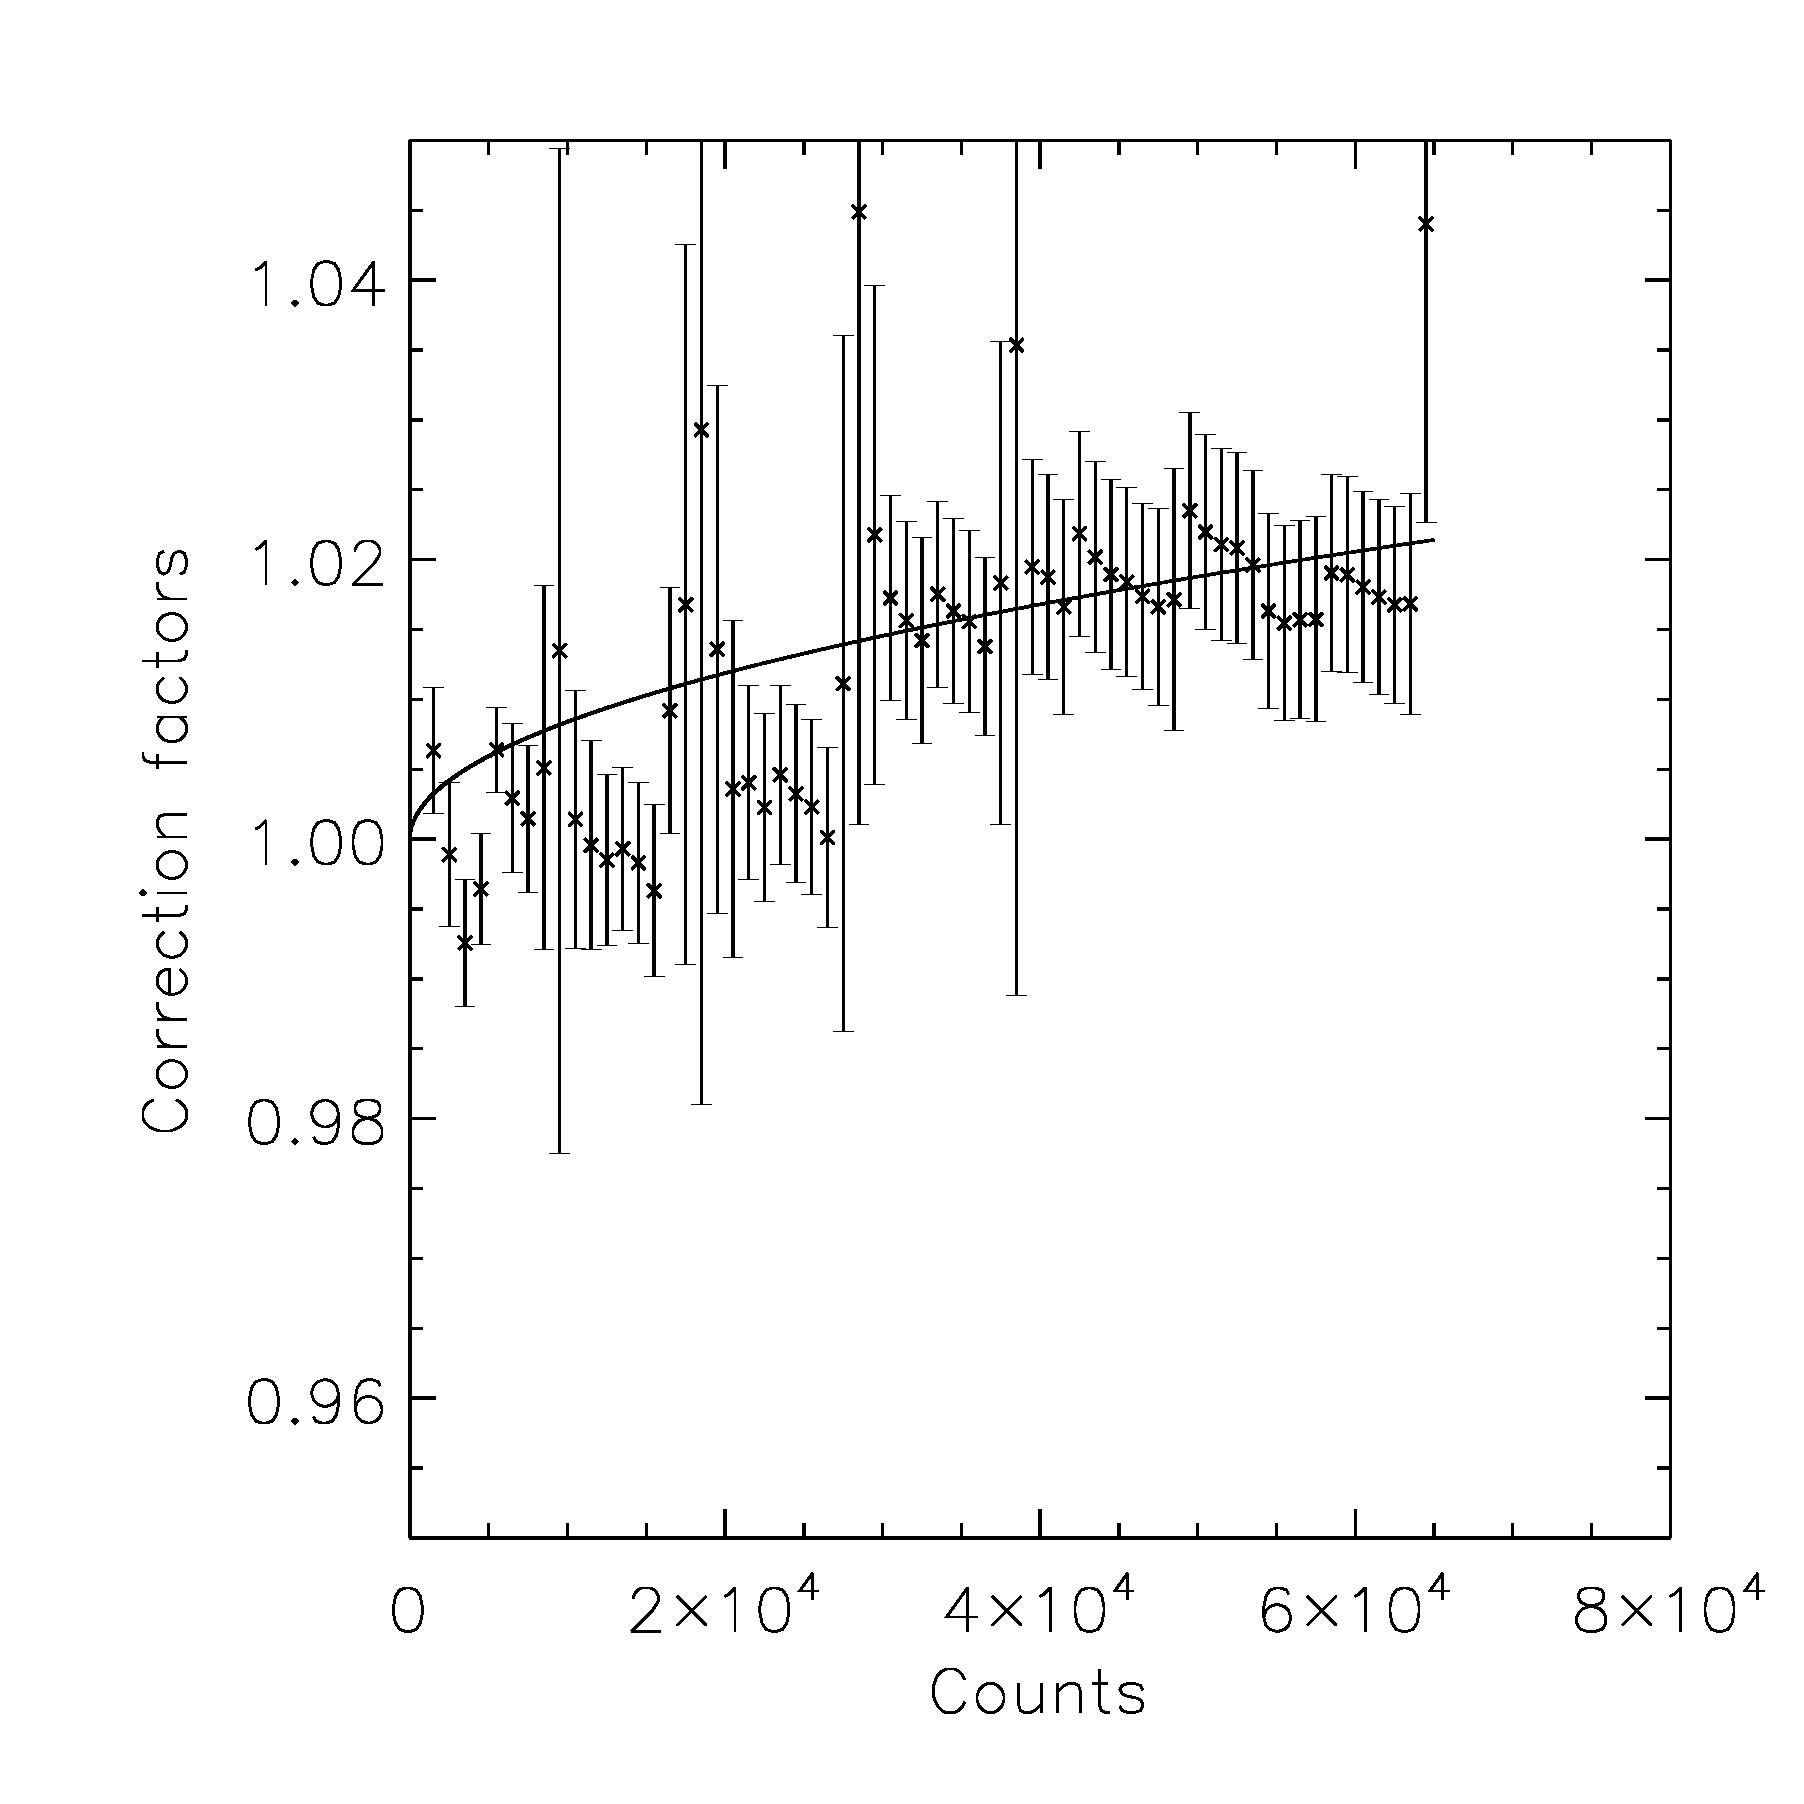
\includegraphics[scale=.25]{sqrt_x.eps}}}
    \hfill
    \subfloat[]{{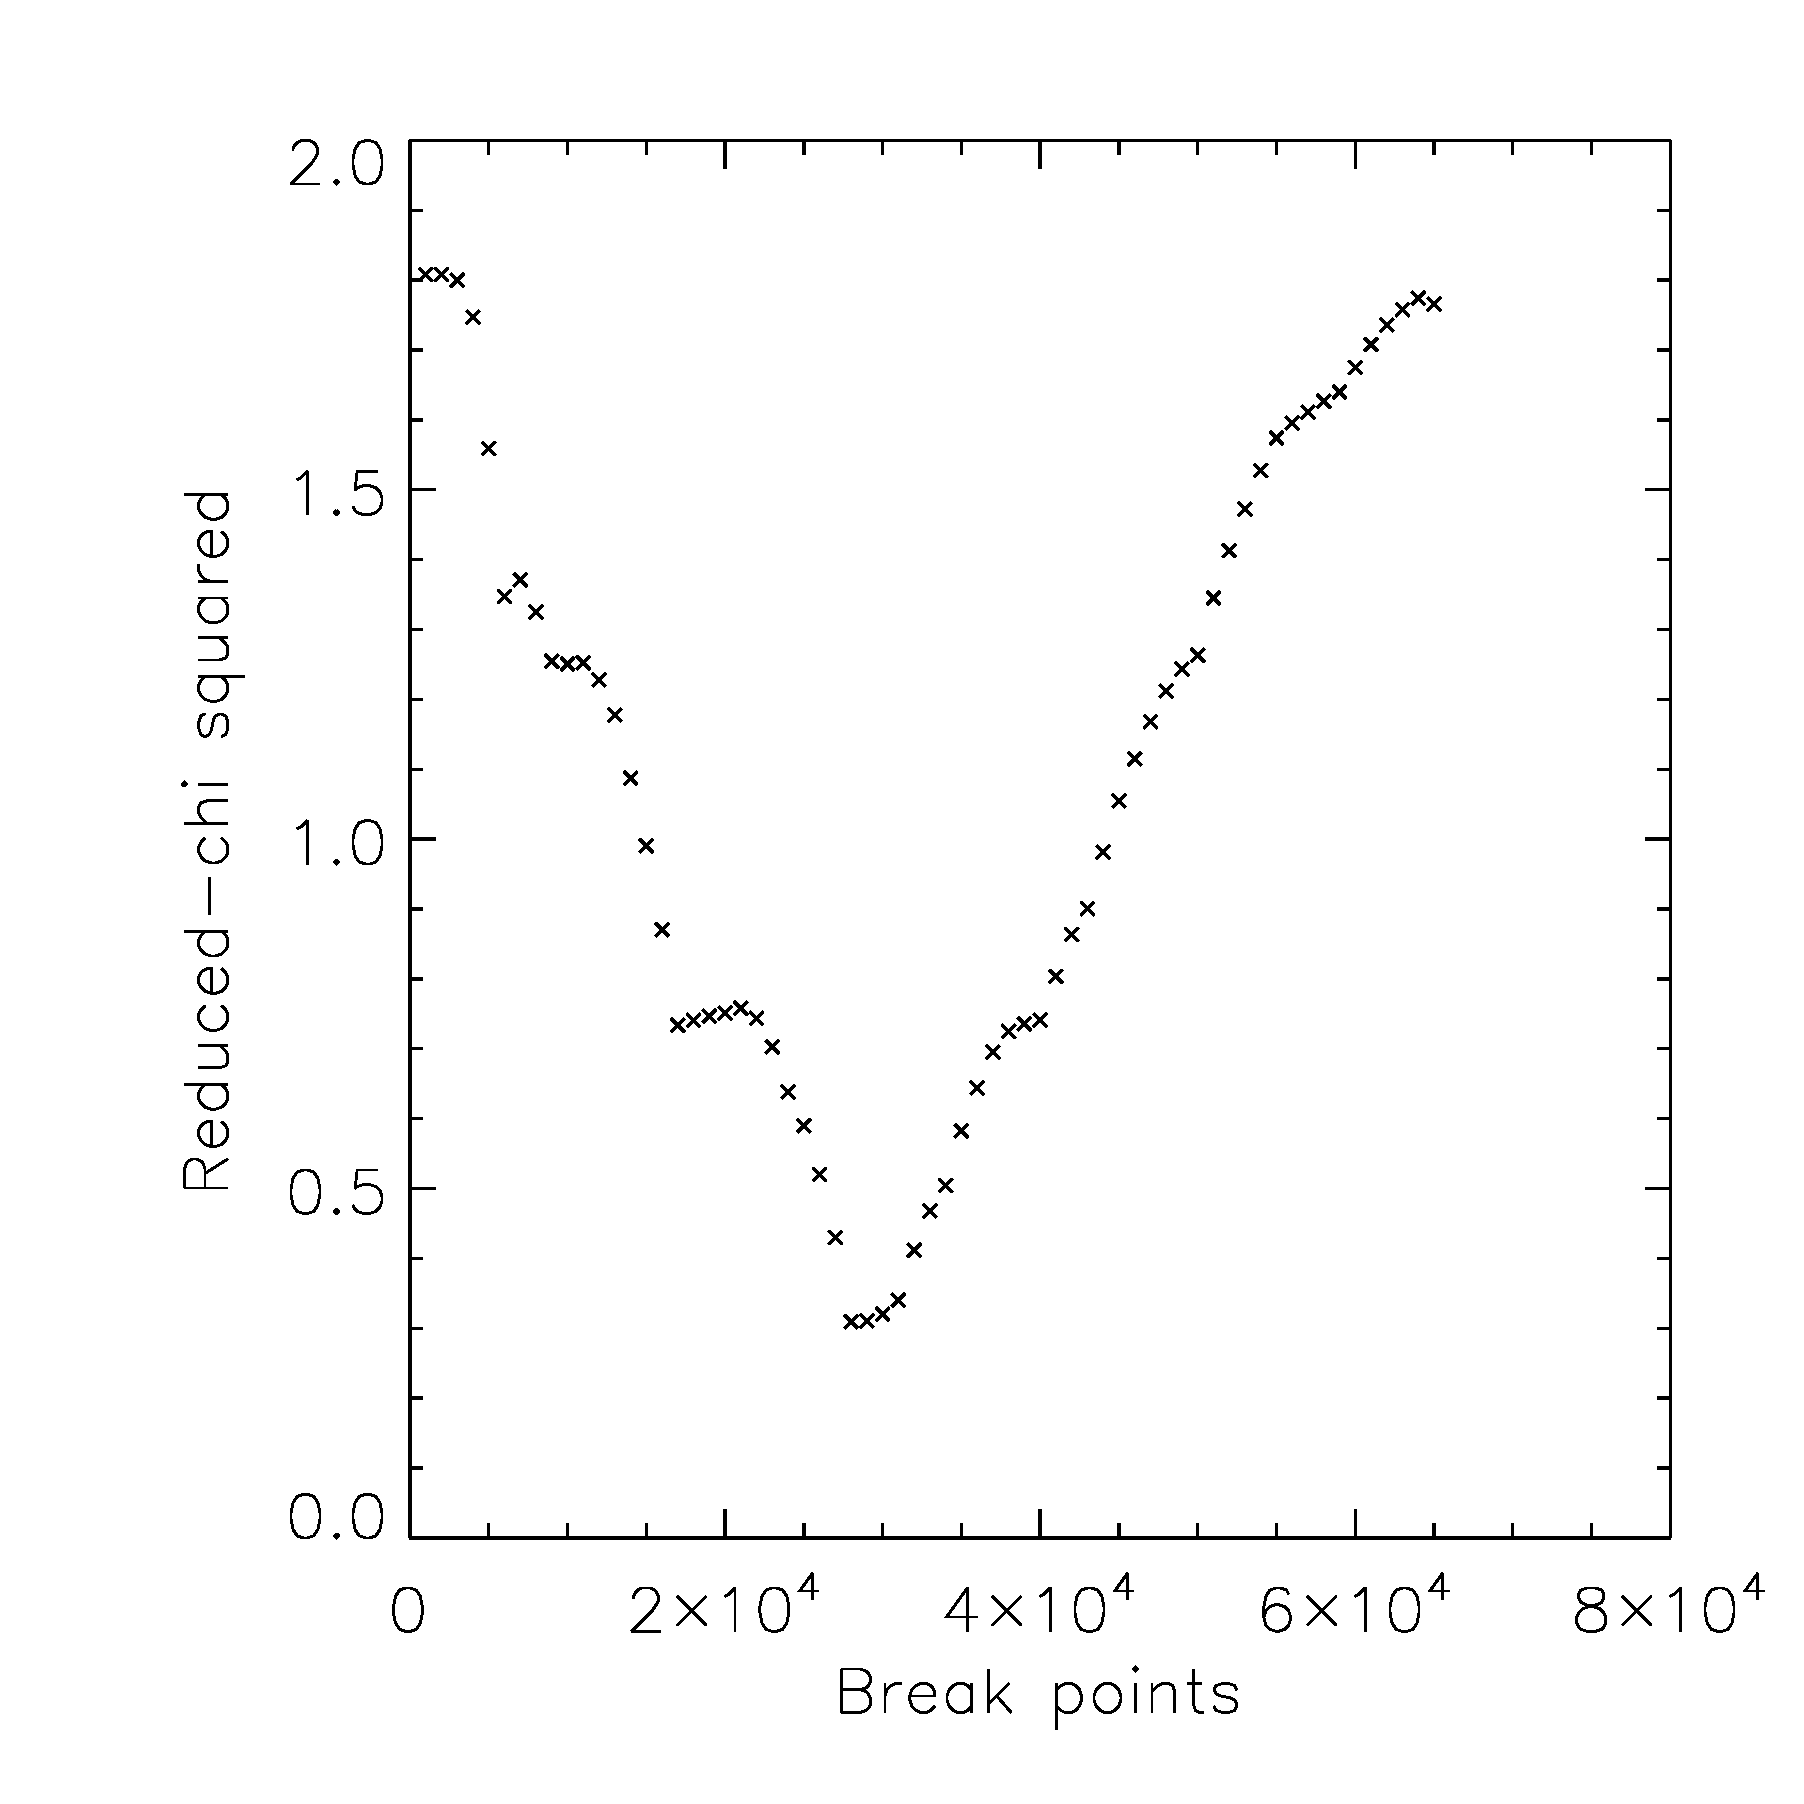
\includegraphics[scale=.25]{min_breakpoint.eps} }}
    \hfill
    \subfloat[]{{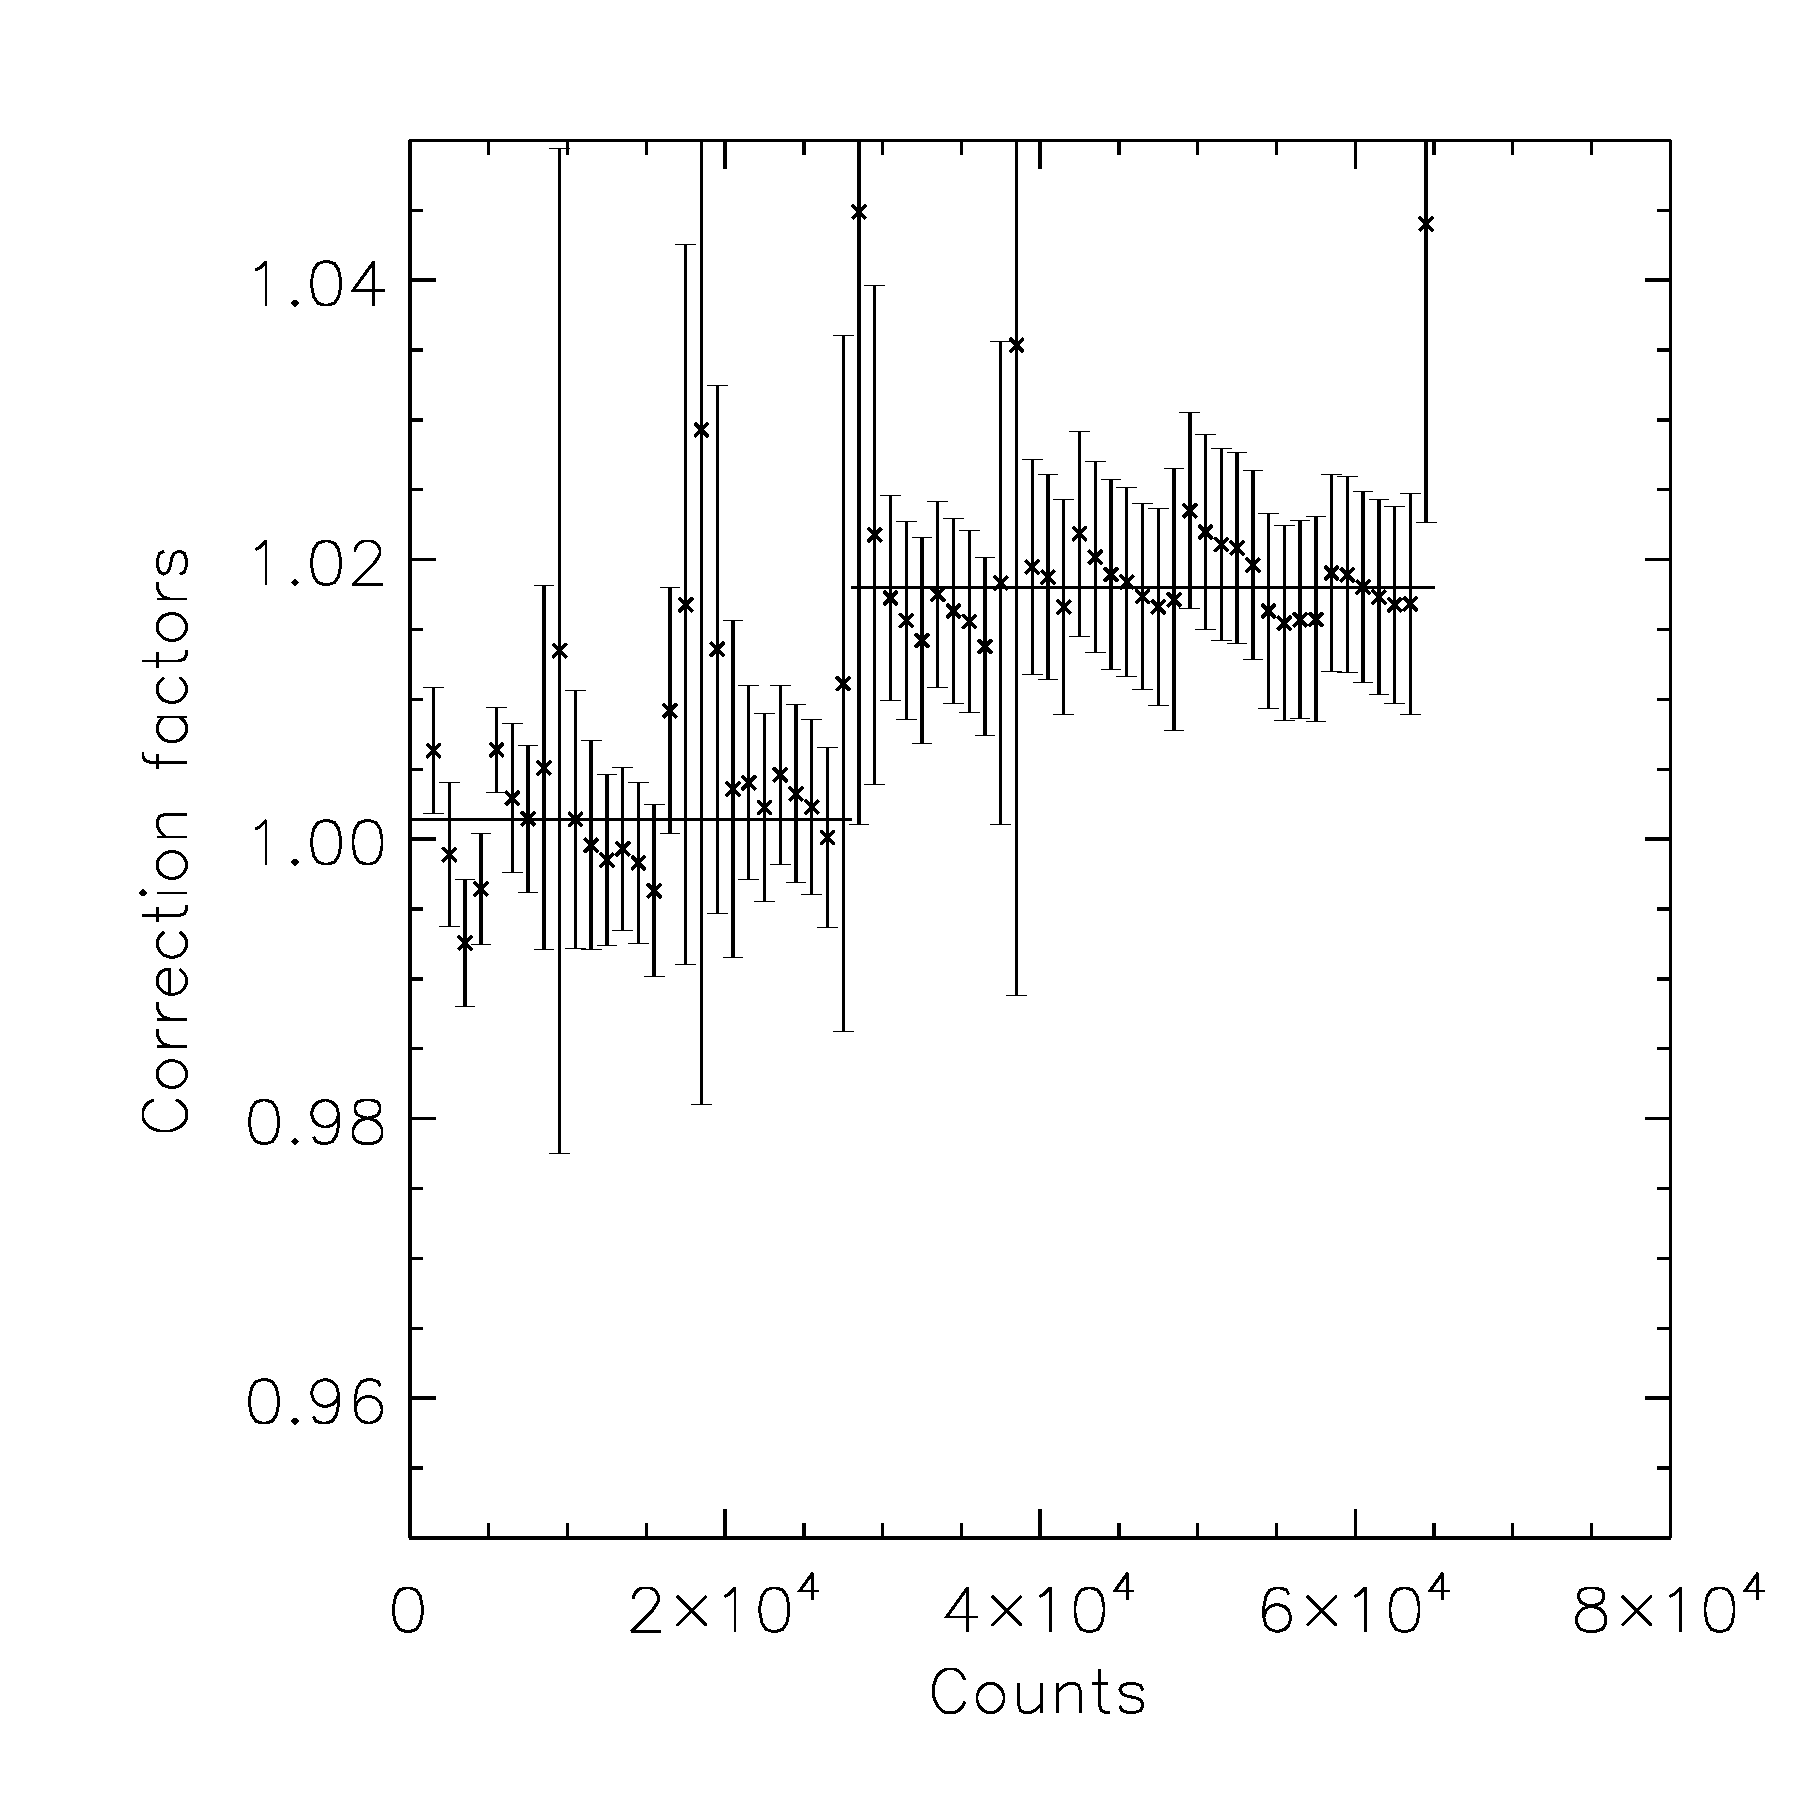
\includegraphics[scale=.25]{piecewise.eps} }}
    \hfill
    \caption{(a) The best-fit line function ${y=(3.777\times10^{-7})x+0.999}$, which was found by fitting a best-fit line to the data points in Figure \ref{fig2} after weighing each data point based on their respective standard deviations, overplotted to our binned correction factors vs measured counts plot in Figure \ref{fig2}. This corresponds to a reduced chi-squared value $\rcs$ of 0.527. (b) The best-fit square root function ${y=(7.053\times10^{-9})\sqrt{x}+1}$ overplotted to our binned correction factors vs measured counts plot in Figure \ref{fig2}. This corresponds to a reduced chi-squared value $\rcs$ of 3.763. Note that to find the best-fit square root function, we first had to linearize the function, before applying the same procedures that we used to find the best-fit line function in Figure 3a. (c) Reduced-chi squared values vs their corresponding break points, where we looped through all possible break points starting from 0 with increments of 1000, and calculated the reduced-chi squared values at each break point using Equations \ref{eq1} and \ref{eq2}. Note that the lowest reduced-chi squared value $\rcs$ is 0.309, at a break point of 28000~counts. (d) The best-fit piecewise function ${y=1.001}$ when ${0<y<28000}$, ${y=1.018}$ when ${28000\leq y<65535}$ overplotted to our binned correction factors vs measured counts plot in Figure \ref{fig2}. We note here that this is the best-fit function out of all the functions where we tested the goodness of their fits, and thus will be the one we use to apply correction factors to any future science images taken using the telescope's camera, i.e. if a given pixel has counts below 28000, we'll increase it by 0.1\%, and if it has counts at or above 28000, we'll increase it by 1.8\%.}
    \label{fig3}
\end{figure}
\clearpage

After overplotting all three functions to our original graph in Figure \ref{fig2} and following the procedures described above, we found that for the best-fit straight line function $y=(3.777\times10^{-7})x+0.999$ in Figure 3a, the reduced-chi squared $\rcs=0.527$; for the best-fit square root function $y=(7.053\times10^{-9})\sqrt{x}+1$ in Figure 3b, $\rcs=3.763$; for the best-fit piecewise function $y=1.001$ when $0<y<28000$, $y=1.018$ when $28000\leq y<65535$ in Figure 3d, we found from the plot in Figure 3c that the break point corresponding to the lowest reduced-chi squared value is at 28000~counts, where $\rcs=0.309$.

Since the piecewise function has the best fit among all the functions tested, as confirmed both by our reduced chi-squared values and by visual inspection of the fits, we will be using it to apply correction factors to any future images taken using the telescope's camera, i.e. if a given pixel has counts below 28000, we'll increase it by 0.1\%, and if it has counts at or above 28000, we'll increase it by 1.8\%.

\end{document}